\documentclass[addpoints]{exam}
\usepackage{amsmath,enumitem,wrapfig}
\usepackage{tikz}
\newcommand{\StudentName}{Sabarno Saha - 22MS037}
\newcommand{\AssignmentName}{Assignment 02}
\pagestyle{headandfoot}
\runningheadrule
\runningheader{PH2101}{\StudentName}{\AssignmentName}
\firstpagefooter{}{}{\thepage}
\runningfooter{}{}{\thepage}
\printanswers
\begin{document}

%starting page
\par\textbf{IISER Kolkata} \hfill \textbf{Assignment 2}
\vspace{3pt}
\hrule
\vspace{3pt}
\begin{center}
        \LARGE{\textbf{PH2101 : Waves and Optics}}
\end{center}
\vspace{3pt}
\hrule
\vspace{4pt}
\textbf{Sabarno Saha}, \textbf{22MS037}\hfill \today
\vspace{20pt}
\bigskip
%starting page end
\begin{questions}
\question 
\textbf{Question 1}
Consider a beaded string of $N$ beads each of mass $m$ (approximated as a long chain of spring-
mass system as shown in the figure). The beads are uniformly placed on the string and the
string has a uniform tension $T$ . The horizontal distance between any two beads in equilibrium
is a. The unstretched lengths of the springs are negligible.\\ \\ 
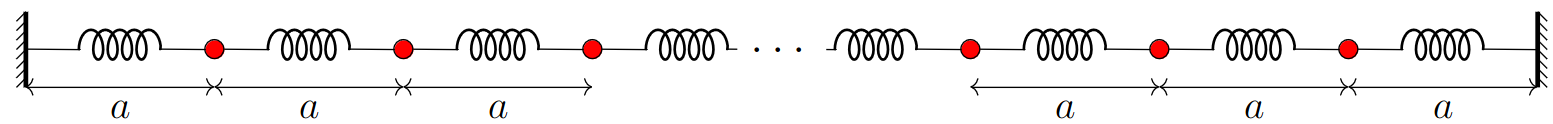
\includegraphics[width = 6.0in]{q1.png}\\ 
(a) Find the equation of the motion of $n^{th}$ bead for the longitudinal mode of vibration
\begin{solution}
 
\end{solution}
(b) Assuming normal mode vibration, find the normal mode frequency $\omega_m$ for $m^{th}$ mod
\begin{solution}
 
\end{solution}
(c) Find the amplitudes of the beads in $m^{th}$ mode ($A^{(m)}_n$ using the notation used in the class).
\begin{solution}
 
\end{solution}
(d) Plot the dispersion relation $\omega$ versus $k$.
\begin{solution}
 
\end{solution}
(e) Check whether we have $\omega_{N+2} = \omega_N$?
\begin{solution}
 
\end{solution}
(f) Check whether we have $A^{(N +2)}_n = A^{(N)}_n$?
\begin{solution}
 
\end{solution}
(g) Qualitatively plot $A^{(1)}_n$ and $A^{(N)}_n$ for all $n$.
\begin{solution}
 
\end{solution}

\question\textbf{Question 2}
Consider two pendulums, $a$ and $b$, with the same string length $L$, but with different bob masses, $M_a$ and $M_b$. They are coupled by a spring of spring constant $K$ which 
is attached to the bobs. Assuming small angle oscillations, \\ \\ 
(a) Find the equations of motion using angles of the pendulums (w.r.t. the vertical) as dynamical variables.
\begin{solution}
 
\end{solution}
(b) Find the normal modes and the normal frequencies
\begin{solution}
    
\end{solution}
(c) For $M_a=M_b=M$, does this reduce to the case considered in class?
\begin{solution}
    
\end{solution}
\question\textbf{Question 3}
Consider the following string with the given configuration.\\
(a)Find the Fourier series representation of the string. You should use the sine representation for the string and not the full representation.\\ 
\begin{center}
    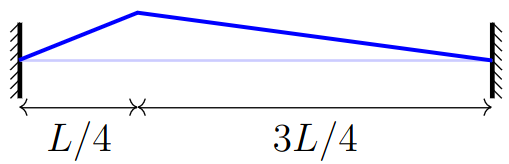
\includegraphics[width = 5.0in]{q2.png}
\end{center}
\begin{solution}
    
\end{solution}
(b) Show that normal modes having nodes at L/4 are absent.
\begin{solution}
 
\end{solution}
(c) Check numerically that your solution matches with the given shape. You may submit
your codes.
\begin{solution}
 
\end{solution}

\question \textbf{ Question 4}
Consider the following pattern. Find the Fourier representation of this pattern. Use the
complete representation (using sine and cosine). Also, check numerically that your solution
matches with the given shape. You may submit your codes.\\
\begin{center}
    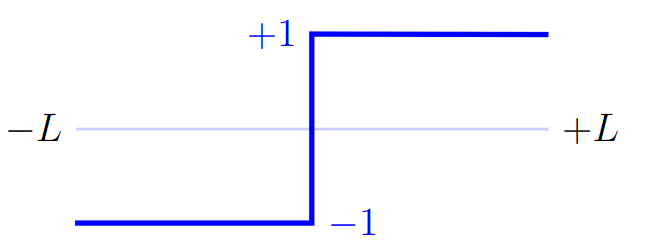
\includegraphics[width = 5.0in]{q4.png}
\end{center}
\begin{solution}
 
\end{solution}

\end{questions}
\end{document}
